\section{Results}

\subsection{Historical Operation of EU Reactors}


\begin{table}[h]
	\centering
	\scalebox{0.86}{
		\begin{tabular}{|c|c|c|}
			\hline
			Category [unit] & Value & Specifics \\ \hline
			Total UOX Usage [t] & 188,196  &  \\ \hline
			Total MOX Usage [t] & 118 & \\ \hline
			Total Spent UOX [t] & 183,807 & \\ \hline
			Total Spent MOX [t] & 0 & All is Reprocessed. \\ \hline
			Total Tailings [t] & 1,125,798 & \\ \hline
		\end{tabular}}
		\caption{Simulation Results}
		\label{tab:sim_result}
		\end {table}

Table \ref{tab:sim_result} lists the important metrics
obtained from the first simulation. The following
values are the EU inventory and history at year 2050.

Tables \ref{tab:eu_num} and \ref{tab:eu_pow} display the
timeseries of number of reactors and installed capacity in EU.



\begin{figure}[htbp!]
	\begin{center}
		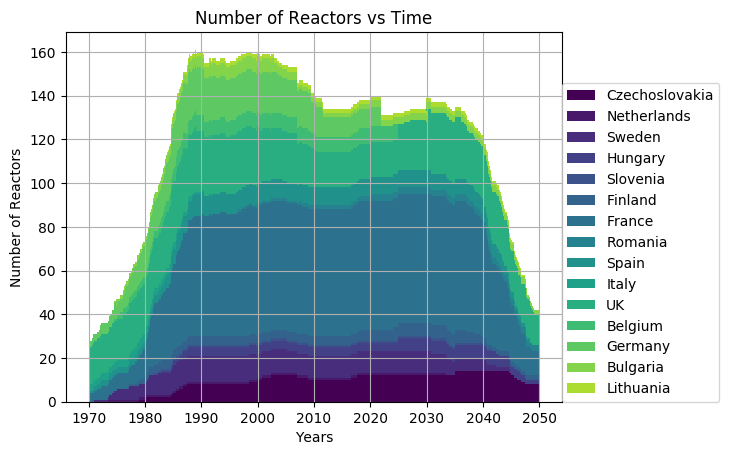
\includegraphics[scale=0.7]{./images/eu_future/number_plot.png}
	\end{center}
	\caption{Timeseries of number of reactors in EU.}
	\label{fig:eu_num}
\end{figure}

\begin{figure}[htbp!]
	\begin{center}
		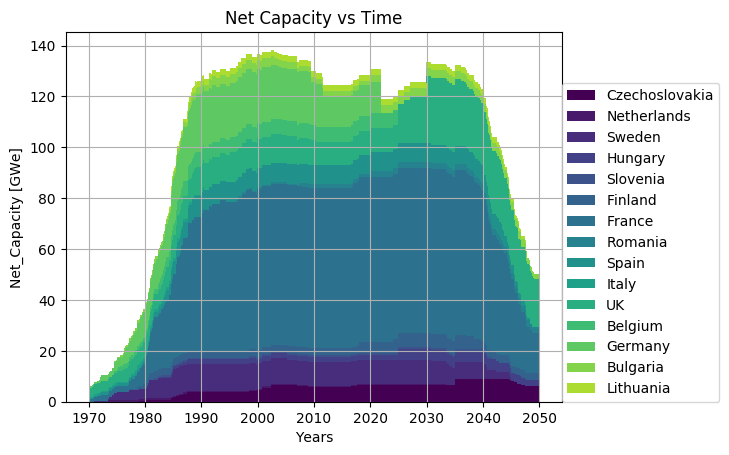
\includegraphics[scale=0.7]{./images/eu_future/power_plot.png}
	\end{center}
	\caption{Timeseries of installed nuclear capacity in EU.}
	\label{fig:eu_pow}
\end{figure}

Figures \ref{fig:eu_tail} and \ref{fig:snf} show the 
timeseries of mass of tailings and spent fuel accumulation in EU.

Figure \ref{fig:eu_fuel} shows the amount of fuel used in EU.
Note that the MOX usage is so little that it is invisible in the
plot. 


\begin{figure}[htbp!]
	\begin{center}
		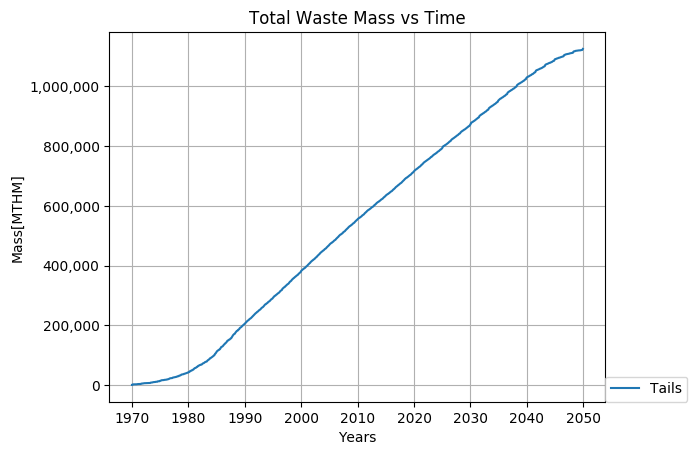
\includegraphics[scale=0.7]{./images/eu_future/tailings.png}
	\end{center}
	\caption{Timeseries of Tailings in the EU.}
	\label{fig:eu_tail}
\end{figure}

\begin{figure}[htbp!]
	\begin{center}
		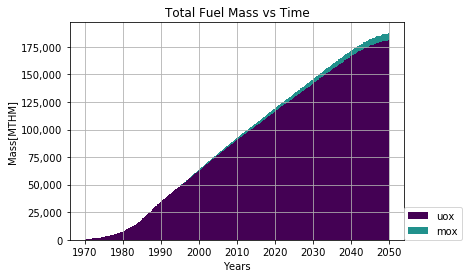
\includegraphics[scale=0.7]{./images/eu_future/total_fuel.png}
	\end{center}
	\caption{Timeseries of total fuel usage in EU.}
	\label{fig:eu_fuel}
\end{figure}


\begin{figure}[htbp!]
	\begin{center}
			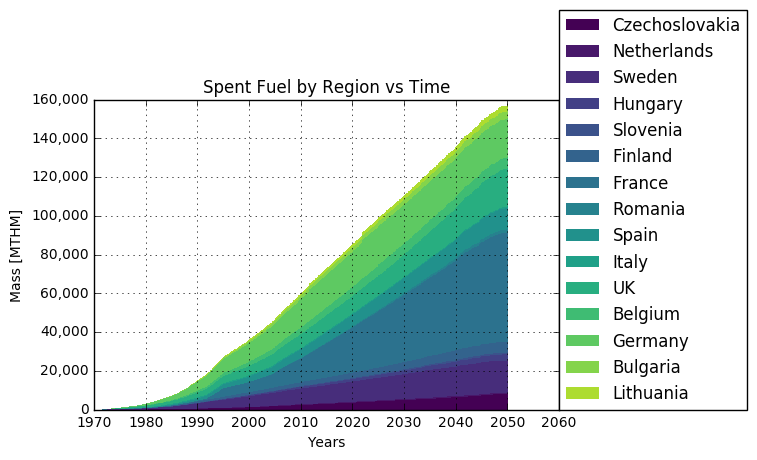
\includegraphics[scale=0.7]{./images/eu_future/snf.png}
	\end{center}
	\caption{Timeseries of Spent Nuclear Fuel in Sink.}
	\label{fig:eu_snf}
\end{figure}

\begin{table}[h]
	\centering
	\begin{tabular}{|c|c|c|}
		\hline
		Isotope & Mass Fraction in Spent Fuel [\%] & Quantity [t] \\ \hline
		Total & .9358 & 1,720 \\ \hline
		Pu238 & .0111 & 20.40 \\ \hline
		Pu239 & .518 & 952.12 \\ \hline
		Pu240 & .232 & 426.43 \\ \hline
		Pu241 & .126 & 231.59 \\ \hline
		Pu242 & .0487 & 89.51 \\ \hline
	\end{tabular}
	\caption{Plutonium From Spent Fuel}
	\label{tab:pu}
\end{table}


To create \gls{MOX}, 10\% Pu and 90\% depleted uranium is used.
Thus $1,720$ tons of plutonium yields $17,200$ tons of
\gls{MOX}. Table \ref{tab:pu} lists the isotope, mass fraction,
and quantity of plutonium that can be obtained from the 2050 \gls{SNF} inventory.


\subsection{French \gls{SFR} Transition Scenario}

From Varaine et al. \cite{marsaultmarie-sophie_pre-conceptual_2012}, a French
ASTRID-type \gls{SFR} of capacity $600 MWe$ needs $1.225$ tons of
plutonium a year, with an initial plutonium loading of $4.9$ tons.
Thus, it can be assumed that the ASTRID reactor takes in $49$ tons of 
\gls{MOX}, and refuels a quarter of its fuel every year. Simply,
an ASTRID reactor needs $12.25$ tons of \gls{MOX} per year. 

The number of SFR-years worth of fuel that can be created with
the \gls{SNF} from 2050 is $\frac{17,611.3 t}{12.25} = 1,437.65 $,
assuming infinite reprocessing and \gls{MOX} fabrication capacity.

However, assuming that \gls{MOX} can be recycled indefinitely,
spent \gls{MOX} from an ASTRID reactor
contains enough plutonium to produce a \gls{MOX} fuel with
the same mass, if mixed with depleted uranium. For example,
spent \gls{MOX} from an ASTRID reactor is 38\% plutonium,
whereas a fresh \gls{MOX} is 10\% plutonium.
The compositions are in appendix table \ref{tab:comp}.
Separating plutonium from spent \gls{MOX} from
an ASTRID reactor can create \gls{MOX} more than
three times the mass of spent \gls{MOX}.

The second scenario, with the tails and spent \gls{UOX}
inventory, evaluates if the French can transition into \gls{SFR}
without constructing additional \gls{LWR}s. This simulation
assumed infinite reprocessing and fabrication capacity.

Figure \ref{fig:fuel} shows the mass of \gls{MOX} used in the 
\gls{SFR}s separated by how they are made, over time.
Note that the mass of \gls{MOX} from the spent \gls{UOX}
stops increasing around 2050, which means that the spent
\gls{MOX} is enough to create the \gls{MOX} for the
\gls{SFR} fleet. 

\begin{figure}[htbp!]
	\begin{center}
		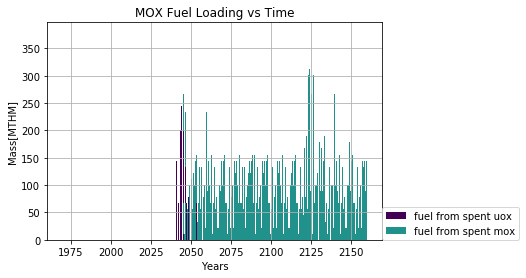
\includegraphics[scale=0.7]{./images/french-transition/where_fuel.png}
	\end{center}
	\caption{Timeseries of fuel used in the \gls{SFR}s [tons]}
	\label{fig:fuel}
\end{figure}

Figure \ref{fig:mox_fab} shows the progression of mox created from
the fabrication plant over time. Figure \ref{fig:mox_fab} shows
the separated plutonium demand from spent \gls{MOX} to fuel the 
ASTRID reactors.

Figure \ref{fig:reprocess_waste} shows the amount of reprocessing waste
(any content from spent fuel other than U, Pu) over time. Note that 
the amount of reprocessing waste is much greater when reprocessing
spent \gls{MOX} from ASTRID reactors, since there is little uranium
or plutonium left due to a high burnup.

\begin{figure}[htbp!]
	\begin{center}
		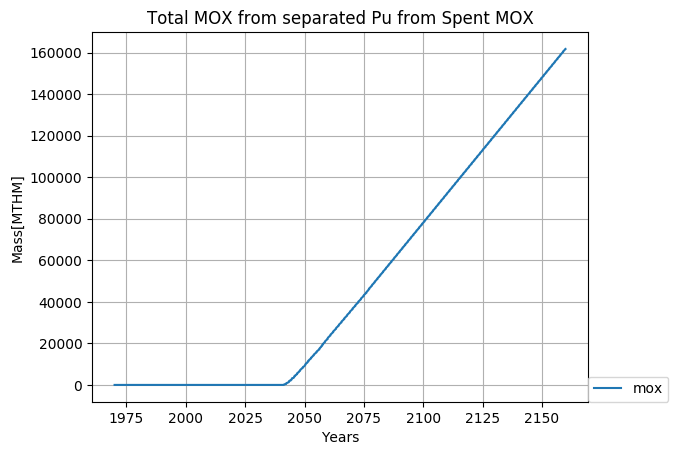
\includegraphics[scale=0.7]{./images/french-transition/mox_from_mixer.png}
	\end{center}
	\caption{Timeseries of MOX produced from Fabrications}
	\label{fig:mox_fab}
\end{figure}


\begin{figure}[htbp!]
	\begin{center}
		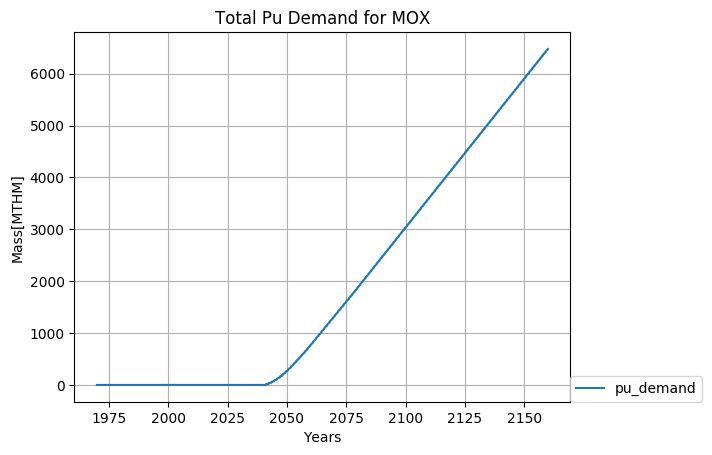
\includegraphics[scale=0.7]{./images/french-transition/pu_demand.png}
	\end{center}
	\caption{Separated Plutonium demand from Spent MOX}
	\label{fig:pu_demand_mox}
\end{figure}

\begin{figure}[htbp!]
	\begin{center}
		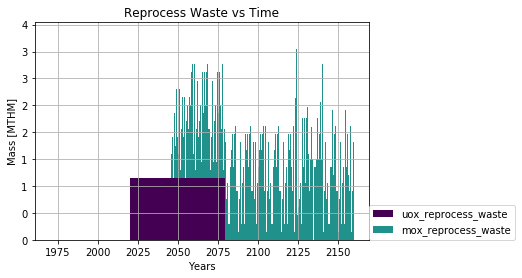
\includegraphics[scale=0.7]{./images/french-transition/reprocess_waste.png}
	\end{center}
	\caption{Reprocessing Waste for French Transition Scenario.}
	\label{fig:reprocess_waste}
\end{figure}


\begin{table}[h]
	\centering
	\scalebox{0.86}{
		\begin{tabular}{|c|c|c|}
			\hline
			Category [unit] & Value & Specifics \\ \hline
			Total MOX used [t] & 164,141 & \\ \hline
			Total MOX from UOX Waste [t] & 2,347.2  &  \\ \hline
			Total MOX from MOX Waste [t] & 161,793.8 & \\ \hline
		\end{tabular}}
		\caption {\gls{SFR} Simulation Results}
		\label{tab:sfr_sim_result}
\end {table}


